\section{Introduction}

\subsection{Rayons cosmiques}
La Terre est constamment bombardée par des rayons cosmiques, majoritairement composés de particules chargées dont des protons et noyaux d'Hélium. Ces particules peuvent atteindre des énergies très importantes ($10^{15}$ à $10^{20}$ eV). Lorsqu'elles pénètrent l'atmosphère, les particules primaires du rayonnement cosmique produisent des particules secondaires instables ayant un temps de vie très court. Ces particules secondaires sont très énergétiques et ultra-relativistes. Elles vont, à leur tour, interagir avec des molécules de l'atmosphère ou se désintégrer en particule plus légère, pour nous donner, entre autre, des muons et des neutrinos.\\

\begin{figure}[h!]
    \center{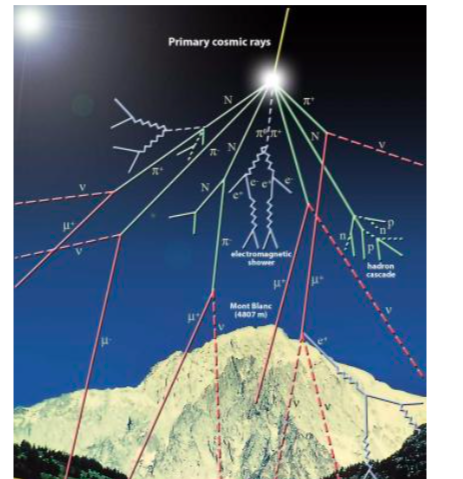
\includegraphics[width=0.56\textwidth]
    {figures/cosmic_rays.png}}
    \caption{\label{fig:CR} Représentation schématique de rayons cosmiques interagissant dans la haute atmosphère.}
\end{figure}

Les muons ainsi produits se propagent jusqu'à la surface de la Terre et sont capables de voyager quelques dizaines de kilomètres sous la surface avant d'interagir. Les neutrinos atmosphériques, quant à eux, peuvent traverser la Terre sans interagir avec un nucléon. Les muons et neutrinos atmosphériques constituent le bruit de fond principal des détecteurs à neutrinos, tel qu'AMANDA et IceCube.

\subsection{Effet Tcherenkov}

L'effet Tcherenkov survient lorsqu'une particule chargée se déplace plus vite que la vitesse de la lumière dans un milieu diélectrique. Ce phénomène résulte de la superposition cohérente d'onde électromagnétique suite à la polarisation du milieu par le passage de la particule chargée.

Si la vitesse de la particule est supérieure au ratio $c/n$ (où $n$ est l'indice de réfraction et $c$ la vitesse de la lumière), il y a formation d'un cône de lumière avec un angle de demi-ouverture $\theta_c$ qui suit la relation:

\begin{equation}
    cos\theta_c = \frac{1}{n\beta}
\end{equation}\\

où $\beta = v/c$, $v$ étant la vitesse de la particule dans le milieu. Le nombre de photons Tcherenkov émis par unité de longueur et de longeur d'onde est donné par la formule de Frank-Tamm: \\

\begin{equation}
     \frac{d^2N}{dx \, d\lambda} = \frac{2\pi \, \alpha}{\lambda^2} \; (1- \frac{1}{n^2 \, \beta^2} )
\end{equation}\\

avec $\alpha$ étant la constante de structure-fine. Comme le nombre de photons produits est inversement proportionnel à la longueur d'onde, la contribution des petites longueurs d'onde est plus importante.

\subsection{Détecteur Tcherenkov}

Compte tenu de leur faible section efficace d'interaction, la détection des neutrinos nécessite un détecteur de grand volume. Cela est réalisé par les détecteurs Tcherenkov en déployant des photo-multiplicateurs (PMs) dans un volume de matériau diélectrique. Chaque PM est contenu dans une bulle de verre sous vide, l'ensemble étant appelé module optique (OM).\\


\begin{figure}[h!]
    \center{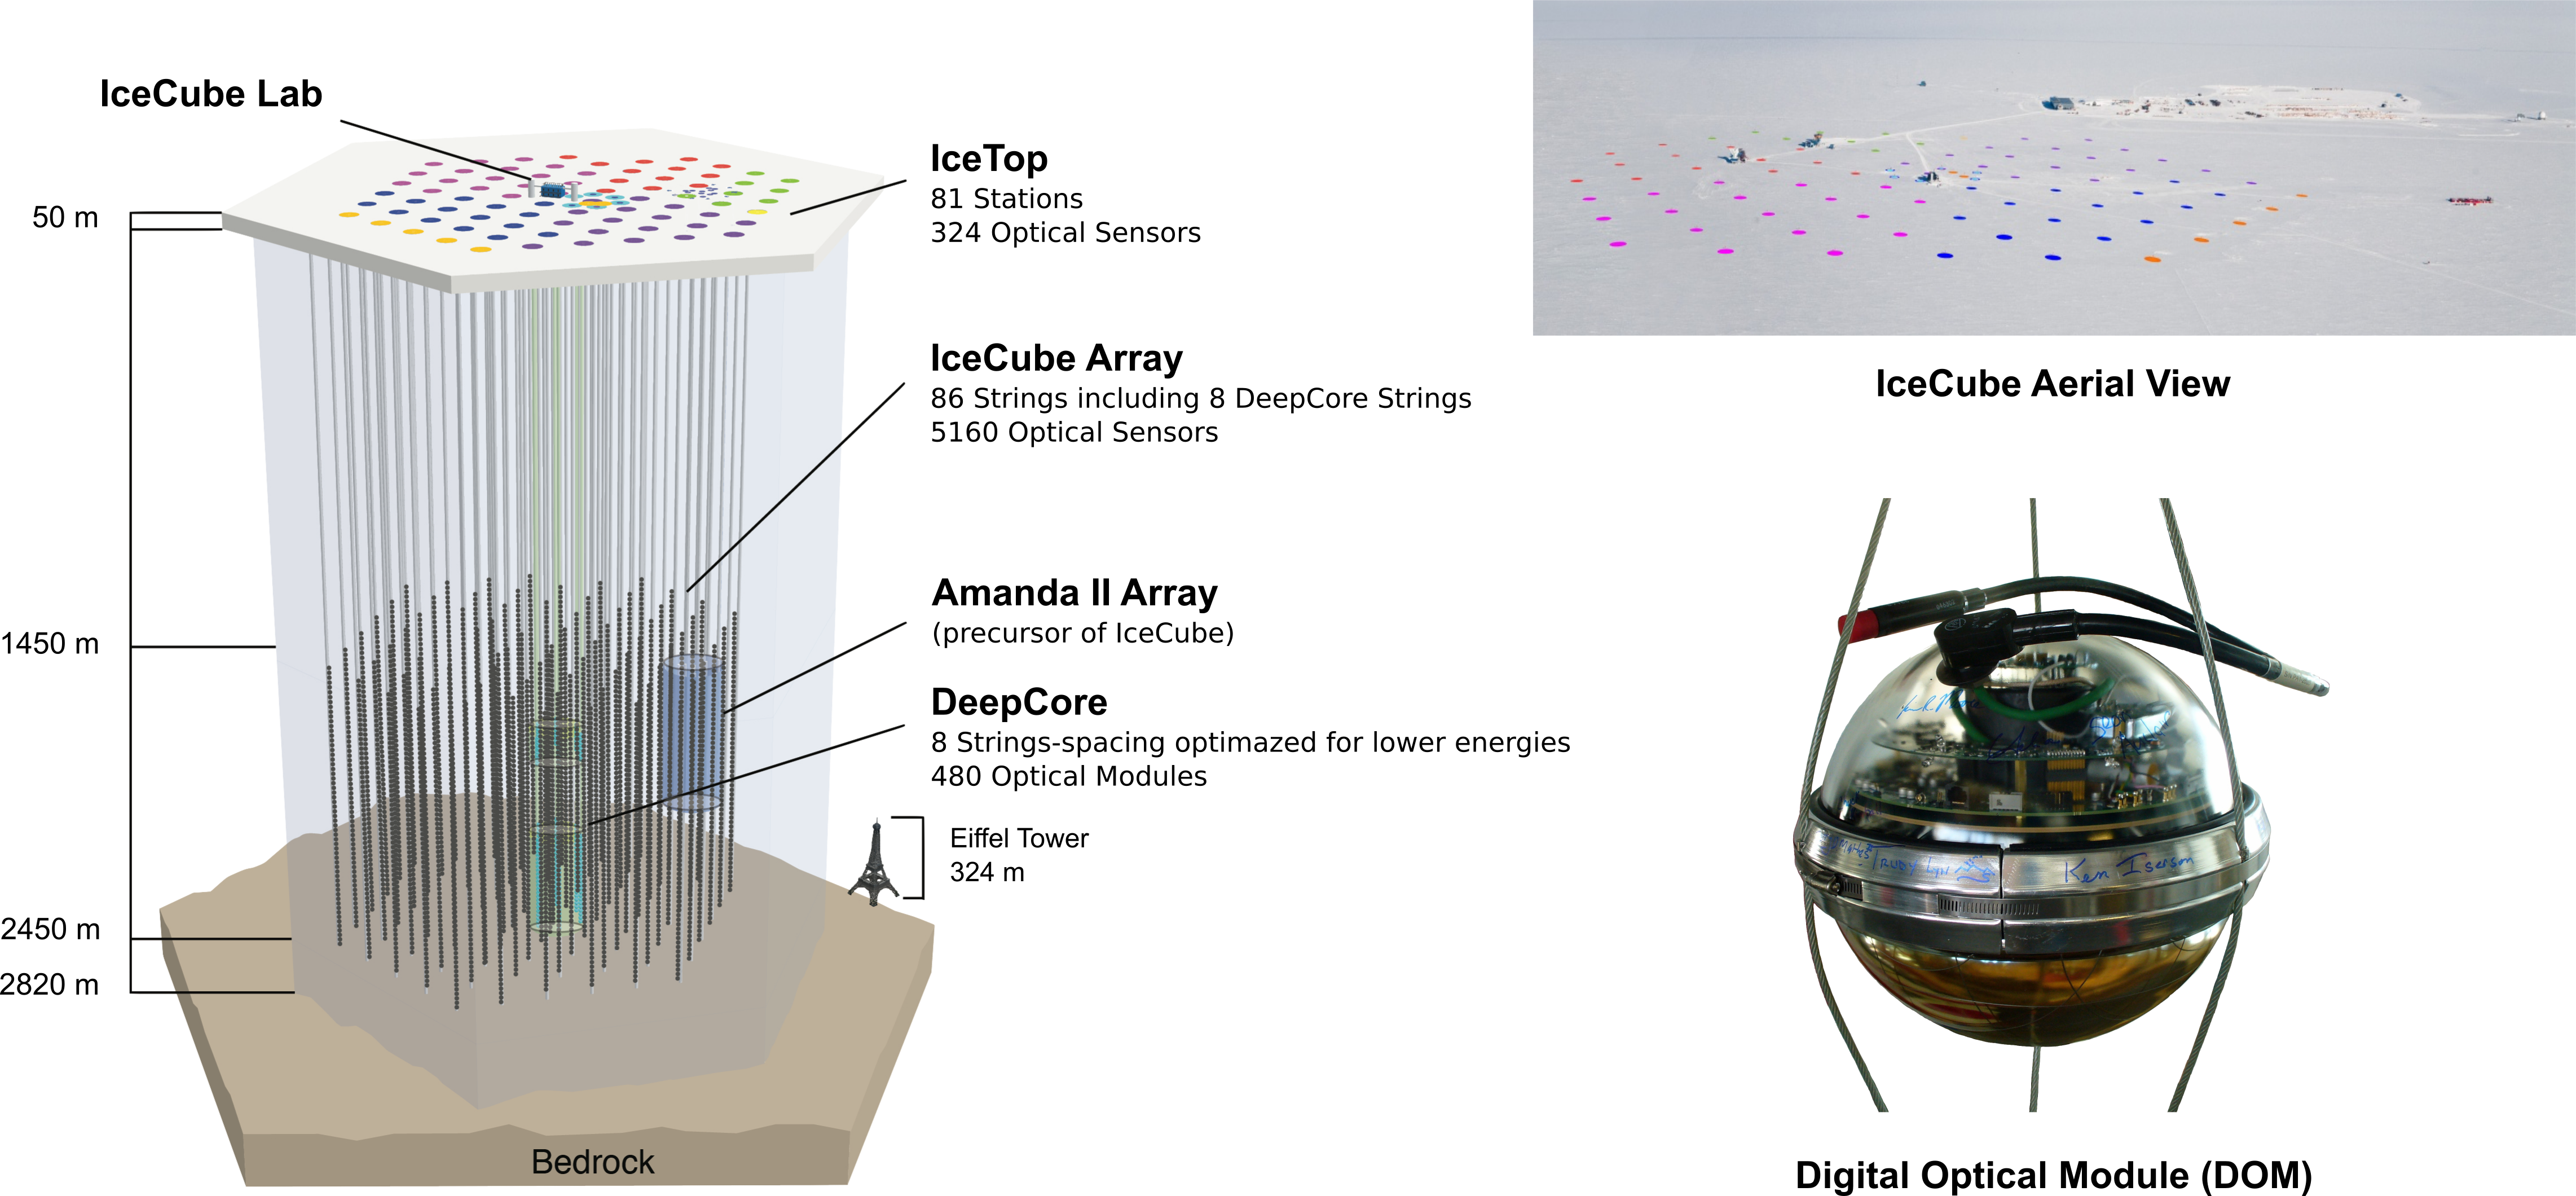
\includegraphics[width=0.8\textwidth]
    {figures/IceCube_Detector.png}}
    \caption{\label{fig:IceCube} Configuration du télescope à neutrinos IceCube.}
\end{figure}


\textbf{AMANDA:}\\
AMANDA (Antarctic Muon and Neutrino Detector Array) est un télescope à neutrino localisé au Pôle Sud. Lors de sa phase finale, le détecteur était composé de 677 modules optiques (OMs) disposés sur 19 câbles. Après 9 ans d'activité, AMANDA a été officiellement incorporé dans au détecteur IceCube en 2005. Ces modules retourne un signal analogique.\\

\textbf{IceCube:}\\
IceCube est un détecteur Tcherenkov d'un kilomètre cube enterré dans la glace du Pôle Sud. Il a pour but principal la détection des neutrinos à haute énergie. IceCube est composé de 5160 modules optiques digitaux (DOMs ou Digital Optical Modules) placés sur 86 câbles.\\

Pour constituer un vaste réseaux d'OMs, il nous faut connaître la réponse de chacun de ceux-ci. La caractérisation de ces modules sera étudiée aux cours de deux manipulations (voir chapitres \ref{sect:Tcherenkov_electron} et \ref{sect:Tcherenkov_muon} ) 